\section{第九周数值分析实验}
\subsection{正交函数族最佳平方逼近}
\begin{ex}
	设 $f(x)=\frac{1}{1+25 x^2}, x \in[-1,1]$, 利用勒让德正交多项式族, 分别构造 $3$ 次, $6$ 次, $10$ 次最佳平方逼近多项式, 并绘图与 $f(x)$ 比较.
\end{ex}
\lstinputlisting[language=matlab]{w9/legendremap.m}
\lstinputlisting[language=matlab]{w9/work9q1.m}
\begin{figure}[H]
	\centering
	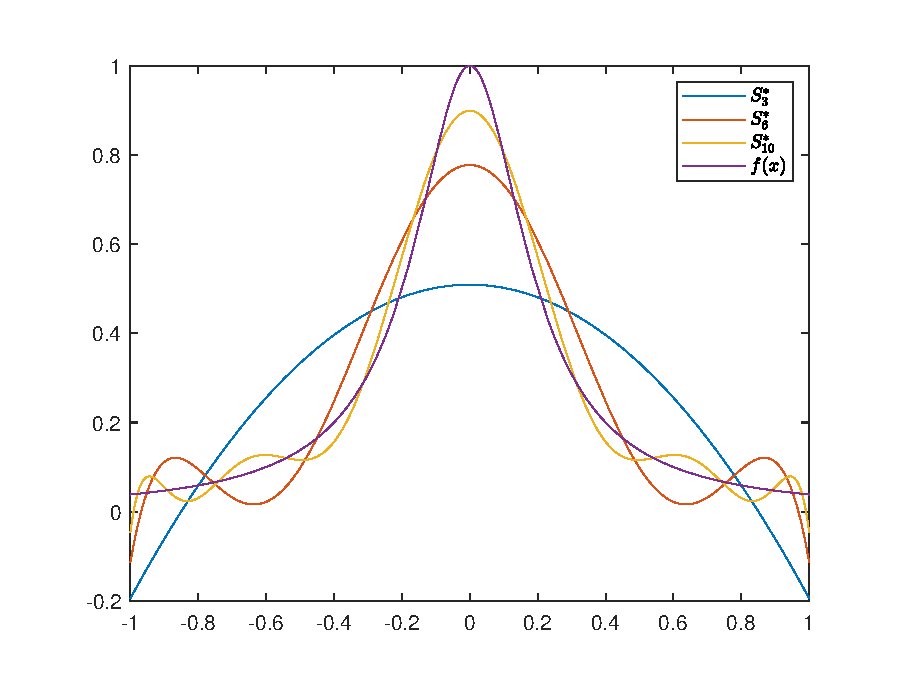
\includegraphics[width = 0.61\linewidth]{w9/figq1.eps}
	\caption{最佳平方逼近}
\end{figure}
\subsection{最小二乘拟合}
\begin{ex}
	实验数据如下
	
	\begin{tabular}{|c|c|c|c|c|c|c|c|c|c|c|c|c|}
		\hline$x_i$ & -1 & -0.8 & -0.6 & -0.4 & -0.3 & -0.1 & 0 & 0.2 & 0.4 & 0.6 & 0.8 & 1 \\
		\hline $y_i$ & 0 & 1.27 & 2.16 & 2.86 & 3.44 & 3.87 & 4.15 & 4.37 & 4.51 & 4.58 & 4.62 & 4.64 \\
		\hline
	\end{tabular}
	
	(1) 确定法方程组, 并求$ 2 $次及$ 3 $次拟合多项式函数 $s=s(x)$;
	
	(2) 与MATLAB拟合工具箱cftool对比.
\end{ex}
\lstinputlisting[language=matlab]{w9/work9q2.m}
\begin{figure}[H]
	\centering
	\subfloat[二次拟合多项式]{\includegraphics[width = 0.5\linewidth]{w9/figq21.eps}}
	\hfill
	\subfloat[三次拟合多项式]{\includegraphics[width = 0.5\linewidth]{w9/figq22.eps}}
	\hfill
	\subfloat[二次拟合多项式]{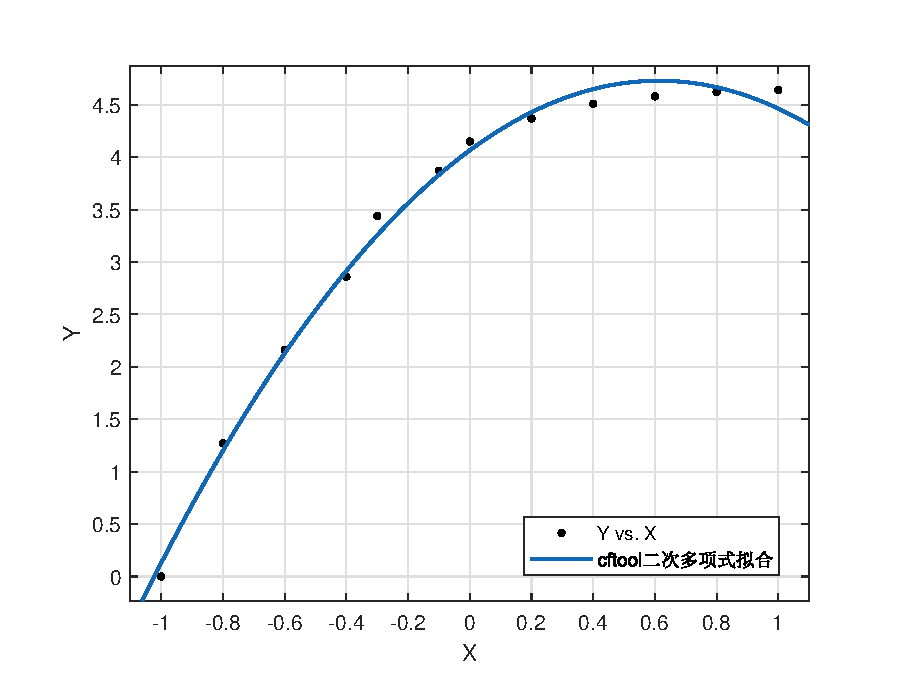
\includegraphics[width = 0.5\linewidth]{w9/figq2c1.eps}}
	\hfill
	\subfloat[三次拟合多项式]{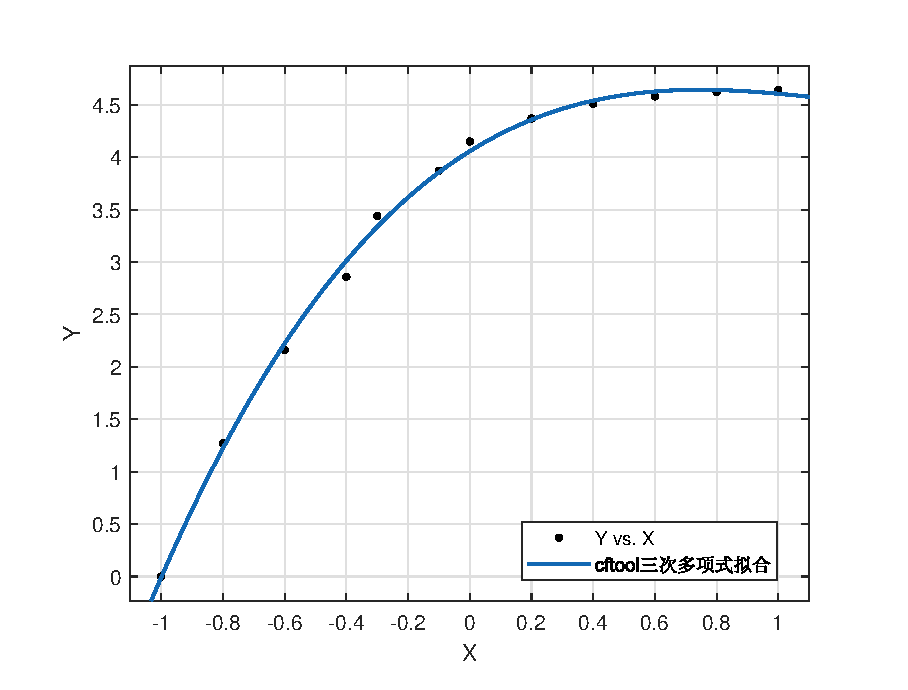
\includegraphics[width = 0.5\linewidth]{w9/figq2c2.eps}}
	\caption{最小二乘拟合}
\end{figure}
